\section{Nombre: Fantasma rojo}   \label{per:fantasmaR}
\subsection{Descripción:}
Alma perdida en el Mictlán. Es un craneo flotate envuelto en una niebla roja.
Se enfrenta al jugador disparándole tonalli negativo para causarle daño. También si toca al jugador le hace daño. 
\subsection{Status:}
Enemigo.
\subsection{Imagen}
Ver figura \ref{fig:fantasmaR}.
\begin{figure}
	\centering
	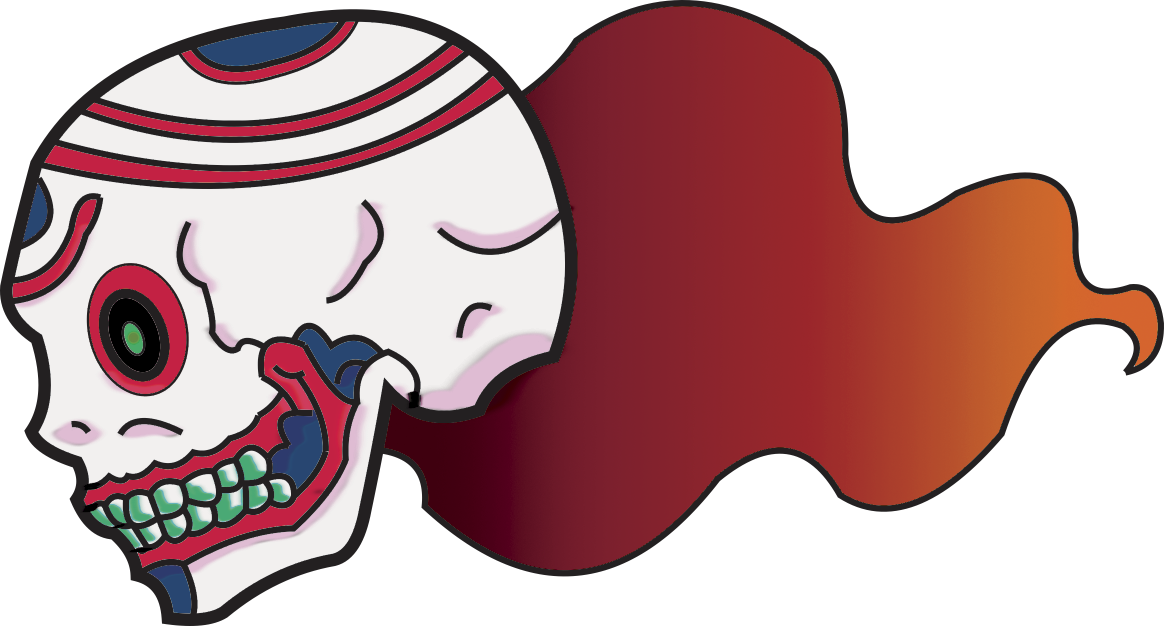
\includegraphics[height=0.2 \textheight]{Imagenes/fantasmaRojo}
	\caption{Fantasma rojo.}
	\label{fig:fantasmaR}
\end{figure} 
\subsection{Encuentro:}
Enemigo de los niveles 2, 3, 6, 7 y 9.
\subsection{Habilidades:}
\begin{itemize}
	\item Disparo rojo. Ver \ref{hab.disparoR}.
	\item Flotar en vertical. Ver \ref{hab.flotarV}.
\end{itemize}
\subsection{Patrón de ataque:}
En un ciclo, realizará la habilidad disparo rojo en todo momento mientras realiza la habilidad flotar en vertical. Este ciclo se repetirá hasta que el enemigo desaparezca.